\documentclass[12pt]{article}
\usepackage{geometry}                % See geometry.pdf to learn the layout options. There are lots.
\geometry{letterpaper}                   % ... or a4paper or a5paper or ... 
%\geometry{landscape}                % Activate for for rotated page geometry
\usepackage[parfill]{parskip}    % Activate to begin paragraphs with an empty line rather than an indent
\usepackage{daves,fancyhdr,natbib,graphicx,dcolumn,amsmath,lastpage,url}
\usepackage{amsmath,amssymb,epstopdf,longtable}
\DeclareGraphicsRule{.tif}{png}{.png}{`convert #1 `dirname #1`/`basename #1 .tif`.png}
\pagestyle{fancy}
\lhead{CE 3372 -- Water Systems Design}
\rhead{FALL 2020}
\lfoot{ES-8}
\cfoot{}
\rfoot{Page \thepage\ of \pageref{LastPage}}
\renewcommand\headrulewidth{0pt}


\begin{document}
\begin{center}
{\textbf{{ CE 3372 -- Water Systems Design} \\ {Exercise Set 8}}}
\end{center}

\section*{\small{Problem Statement and Background}}
Figure \ref{fig:aerial} is an older (circa 1993) aerial image of a portion of Houston, Texas.   
The red polygon is the drainage boundary for a storm sewer system that drains North from the part of the area near Westheimer Road to a tributary of Buffalo Bayou and East from the area.
The drainage ditch is shown as the ``blue''   fuzzy line on the figure.  
Drainage in the ditch is from West to East.
The two main streets in the study area are highlighted in magenta.  
\begin{figure}[h!] %  figure placement: here, top, bottom, or page
   \centering
   \includegraphics[height=5in]{Image118.jpg} 
   \caption{Tanglewilde Drive Study Area}
   \label{fig:aerial}
\end{figure}
\clearpage

Figure \ref{fig:survey} is a map showing storm drainage alignments and inlets location.  
\begin{figure}[h!] %  figure placement: here, top, bottom, or page
   \centering
   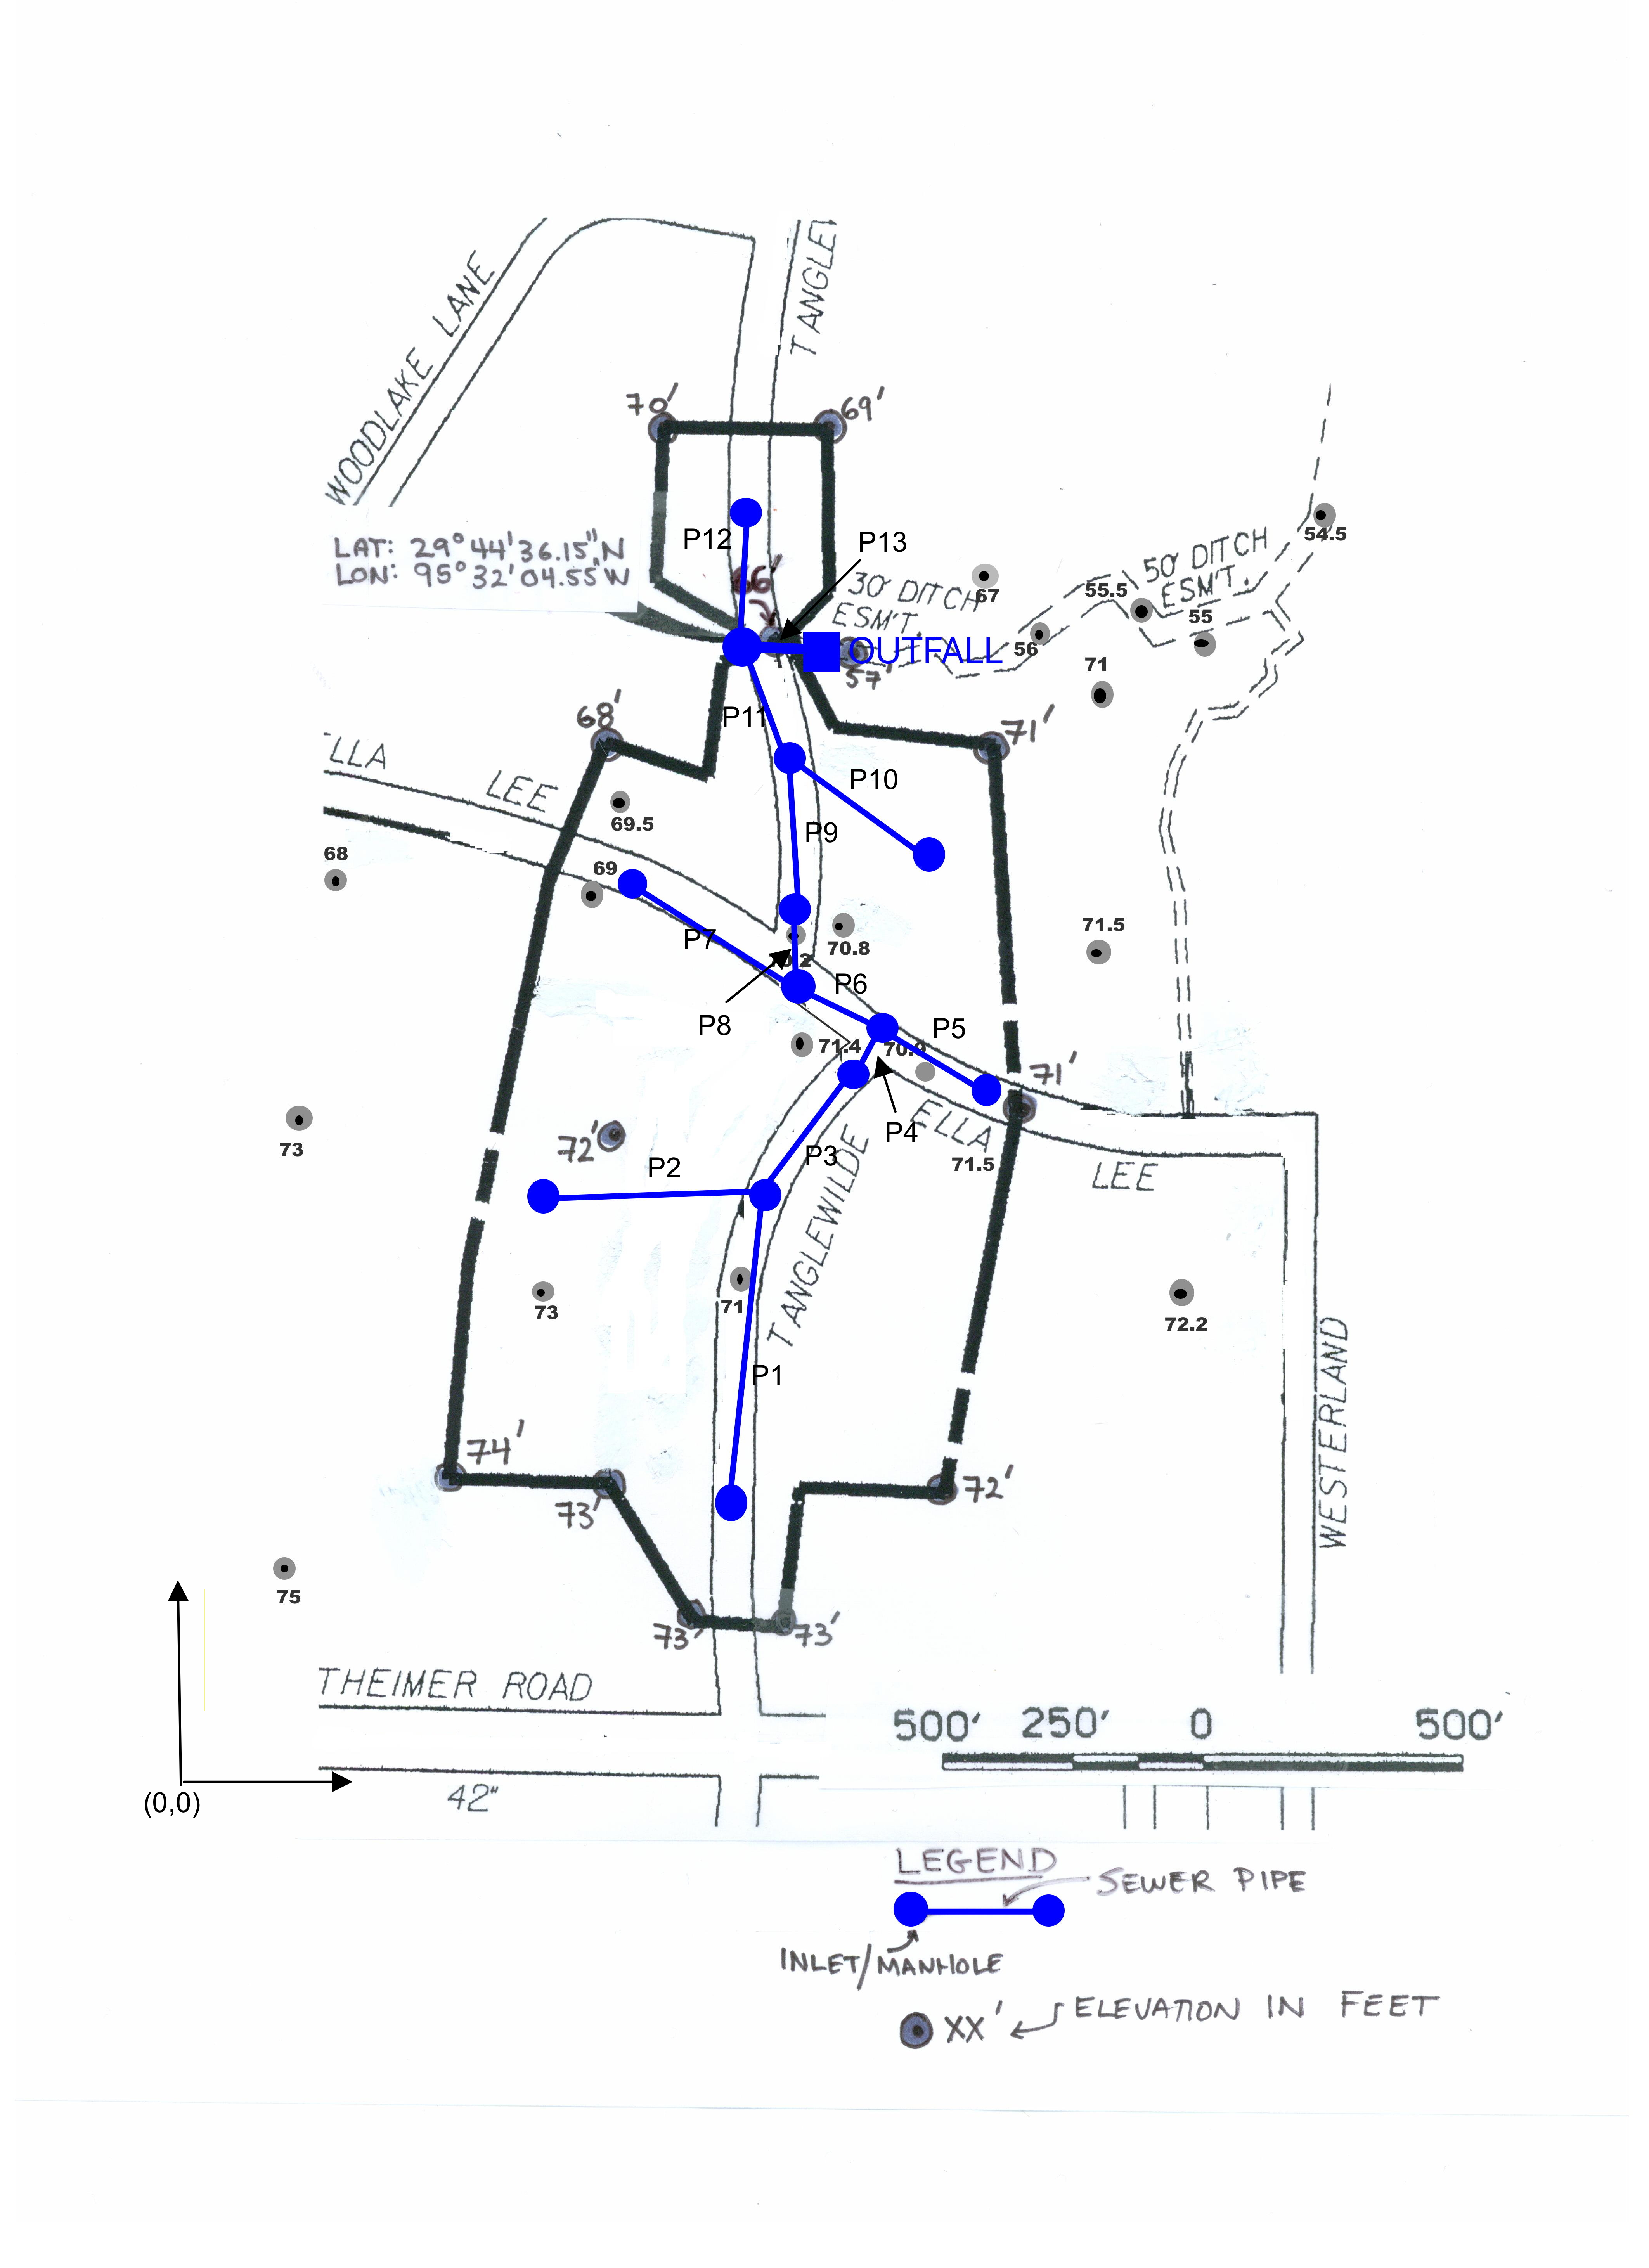
\includegraphics[height=7in]{Image119B.jpg} 
   \caption{Tanglewilde Drive Storm Drain Inlet and Pipe Alignments}
   \label{fig:survey}
\end{figure}

The figure shows land surface elevations in feet at the indicated locations.  
A linear scale is shown in the legend.  
Use the map(s) and:

\begin{enumerate}
\item Apply the rational design method to size the conduits for a 5-year storm, for Harris County, Texas.
\item Specify the invert (flow line) elevations of the nodes (inlets and junction boxes).
\item Specify the soffit (crown) elevations for the pipes at each node.
\end{enumerate}

Submit a memorandum with screen captures of the relevant components above.  Save your work, you need it for Project 2.













 









\end{document}  